% !TEX root = ../enac_project_fr.tex
%%%%%%%%%%%%%%%%%%%%%%%%%%%%%%%%%%%%%%%%%%%%%%%%%%%%%%%%%%%%%%%%%%%%
% Annexe A - Détails des modèles de correction
%%%%%%%%%%%%%%%%%%%%%%%%%%%%%%%%%%%%%%%%%%%%%%%%%%%%%%%%%%%%%%%%%%%%

\chapter{Détails des modèles de correction}
\thispagestyle{fancy}
\label{annexA}


\section{Fonctions de projection troposphérique}
\label{annexe:nmf}

Dans cette étude, les fonctions de projection utilisées pour modéliser le
retard troposphérique sont celles du modèle \textit{Niell Mapping Function}
(NMF), proposé par Niell~\cite{niell1996}. Il sert à déterminer
séparément les facteurs de projection associés aux composantes hydrostatique
et humide du retard troposphérique.

\subsection*{Formulation générale}

Le modèle NMF utilise deux fonctions de projection distinctes,
$M_{\mathrm{dry}}$ et $M_{\mathrm{wet}}$, permettant de projeter les retards
zénithaux hydrostatique et humide dans la direction du satellite :

\begin{align}
T(E)
&=
M_{\mathrm{dry}}(E)\,ZHD
+
M_{\mathrm{wet}}(E)\,ZWD,
\end{align}

où $E$ est l'angle d'élévation du satellite, $ZHD$ le retard hydrostatique
zénithal et $ZWD$ le retard humide zénithal.

Les deux fonctions reposent sur une fonction élémentaire $m(E,a,b,c)$,
correspondant à la fonction de projection de Marini normalisée à l'unité au
zénith :

\begin{align}
m(E,a,b,c)
&=
\frac{
1+\dfrac{a}{1+\dfrac{b}{1+c}}
}{
\sin E+
\dfrac{a}{\sin E+\dfrac{b}{\sin E+c}}
}.
\label{eq:marini_mapping}
\end{align}

Les coefficients $a$, $b$ et $c$ sont différents selon la composante
troposphérique considérée.

\subsection*{Fonction de projection hydrostatique}

La fonction de projection hydrostatique est donnée par

\begin{align}
M_{\mathrm{dry}}(E,H)
&=
m(E,a_d,b_d,c_d)
+
\Delta m(E,H),
\label{eq:nmf_hydrostatic}
\end{align}

avec une correction liée à l'altitude du récepteur :

\begin{align}
\Delta m(E,H)
&=
\left[
\frac{1}{\sin E}
-
m(E,a_{ht},b_{ht},c_{ht})
\right]H,
\label{eq:nmf_height}
\end{align}

où $H$ est la hauteur du récepteur, exprimée en kilomètres.
Les paramètres $a_d$, $b_d$ et $c_d$ sont les coefficients de la composante
hydrostatique, tandis que $a_{ht}$, $b_{ht}$ et $c_{ht}$ sont les coefficients
utilisés pour la correction d'altitude~\cite{niell1996}.

Les coefficients hydrostatiques dépendent de la latitude du récepteur et,
pour tenir compte de la variation saisonnière de l'atmosphère, du temps.
Pour chacun des coefficients $\xi \in \{a_d,b_d,c_d\}$, cette dépendance est
décrite par

\begin{align}
\xi(\varphi,t)
&=
\xi_{\mathrm{avg}}(\varphi)
-
\xi_{\mathrm{amp}}(\varphi)
\cos\left(
2\pi\frac{t-T_0}{365.25}
\right),
\label{eq:nmf_time}
\end{align}

où $\varphi$ est la latitude géographique du récepteur, $t$ le temps écoulé
depuis le 1 janvier de l'année considérée, exprimé en jours, et $T_0=28$
correspond au 28e jour de l'année.

Les valeurs de $\xi_{\mathrm{avg}}$ et $\xi_{\mathrm{amp}}$ sont obtenues par
interpolation linéaire entre les deux latitudes tabulées encadrant la
latitude du récepteur. Les coefficients $a_{ht}$, $b_{ht}$ et $c_{ht}$ sont,
quant à eux, donnés par les valeurs tabulées.

\subsection*{Fonction de projection humide}

La fonction de projection associée à la composante humide est plus
simplement donnée par

\begin{align}
M_{\mathrm{wet}}(E)
&=
m(E,a_w,b_w,c_w),
\label{eq:nmf_wet}
\end{align}

où $a_w$, $b_w$ et $c_w$ sont les coefficients associés à la composante
humide.

Contrairement aux coefficients hydrostatiques, ces coefficients ne dépendent
que de la latitude du récepteur. Ils sont obtenus par interpolation linéaire
entre les valeurs tabulées correspondant aux latitudes voisines.

\subsection*{Coefficients du modèle}

Les coefficients utilisés par le modèle NMF sont donnés dans les tableaux
suivants.


\begin{figure}[H]

    \centering

    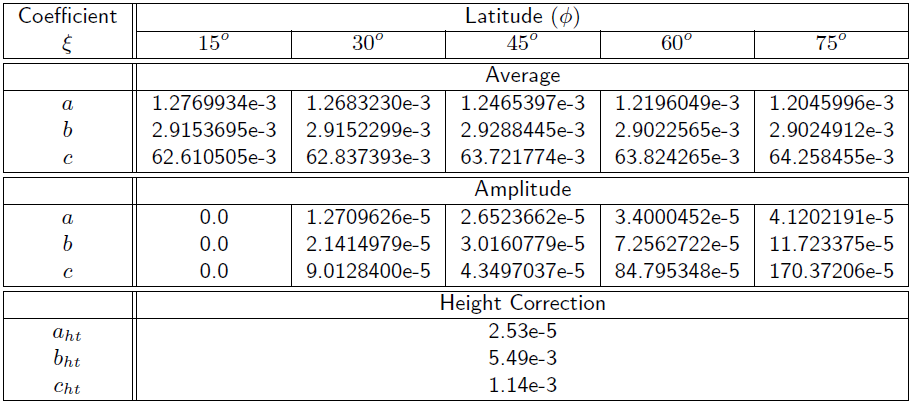
\includegraphics[width=0.75 \linewidth]{images/Niell_Mapping_Table_1.png}

    \caption[Tableau des coefficients du modèle NMF pour la fonction
    hydrostatique.]{Tableau des coefficients du modèle NMF pour la fonction
    hydrostatique. Source :
    \href{https://gssc.esa.int/navipedia/index.php/Mapping_of_Niell}{Navipedia,
    \textit{Mapping of Niell}}.}

    \label{fig:nmf_hydrostatic}

\end{figure}

\begin{figure}[H]

    \centering

    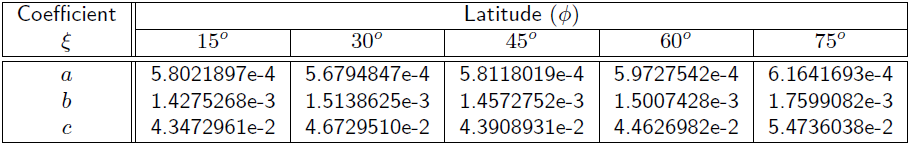
\includegraphics[width=0.75 \linewidth]{images/Niell_Mapping_Table_2.png}

    \caption[Tableau des coefficients du modèle NMF pour la fonction
    humide.]{Tableau des coefficients du modèle NMF pour la fonction humide.
    Source :
    \href{https://gssc.esa.int/navipedia/index.php/Mapping_of_Niell}{Navipedia,
    \textit{Mapping of Niell}}.}

    \label{fig:nmf_wet}

\end{figure}


\section{Modèle ionosphérique de Klobuchar} \label{Klobuchar}

Le modèle de Klobuchar est un modèle empirique de correction du retard
ionosphérique diffusé dans le message de navigation GPS et fournit une estimation
du retard ionosphérique à partir de huit coefficients $\alpha_i$ et
$\beta_i$ transmis par les satellites GPS~\cite{klobuchar1987}.

Le modèle suppose que les électrons responsables du retard ionosphérique sont
concentrés dans une couche mince située à une altitude d'environ $350$~km.
Le retard selon la ligne de visée est alors obtenu à partir du retard
vertical au point de percement ionosphérique (\textit{Ionospheric Pierce
Point}, IPP), auquel est appliqué un facteur de projection dépendant de
l'élévation du satellite

\subsection{Calcul du point de percement ionosphérique}

Le modèle utilise la position géodésique du récepteur ainsi que l'élévation
et l'azimut du satellite afin de déterminer le point de percement de la ligne
de visée avec la couche ionosphérique.

On note $\varphi_u$ et $\lambda_u$ respectivement la latitude et la longitude
géodésiques du récepteur. Les coordonnées du récepteur sont exprimées en
\textit{semi-cercles} dans la formulation originale du modèle.

La latitude géomagnétique du point de percement, notée $\varphi_m$, est
ensuite déterminée à partir de la latitude du point de percement et de la
position du pôle magnétique utilisée par le modèle.

Cette latitude géomagnétique constitue la variable d'entrée des polynômes
permettant de déterminer l'amplitude et la période de la variation
diurne du retard ionosphérique.

\subsection{Amplitude et période du modèle}

L'amplitude du retard ionosphérique est déterminée à partir des quatre
coefficients $\alpha_0,\ldots,\alpha_3$ diffusés dans le message de navigation :

\begin{align}
A_I
=
\sum_{n=0}^{3}\alpha_n\varphi_m^n.
\label{eq:klobuchar_amplitude}
\end{align}

Si la valeur obtenue est négative, l'amplitude est fixée à zéro.

De manière analogue, la période de la variation diurne est calculée à partir
des coefficients $\beta_0,\ldots,\beta_3$ :

\begin{align}
P_I
=
\sum_{n=0}^{3}\beta_n\varphi_m^n.
\label{eq:klobuchar_period}
\end{align}

Lorsque la valeur calculée est inférieure à $72000$~s, elle est remplacée
par cette valeur minimale.

La phase de la variation diurne est alors définie par

\begin{align}
X_I
=
\frac{2\pi(t-50400)}
{P_I},
\label{eq:klobuchar_phase}
\end{align}

où $t$ est le temps GPS exprimé en secondes dans la journée. La valeur
$50400$~s correspond à $14$~h, instant autour duquel le maximum de la
variation diurne est supposé se produire.

\subsection{Retard ionosphérique vertical}

Le retard ionosphérique vertical sur la fréquence GPS L1 est alors modélisé
par une fonction périodique. Lorsque $|X_I|\leq 1.57$, cette fonction est
approchée par les premiers termes du développement limité du cosinus :

\begin{align}
I_{\mathrm{vert,L1}}
=
5\times10^{-9}
+
A_I
\left(
1-\frac{X_I^2}{2}
+\frac{X_I^4}{24}
\right).
\label{eq:klobuchar_vertical}
\end{align}

Lorsque $|X_I|>1.57$, le retard vertical est fixé à sa valeur nocturne :

\begin{align}
I_{\mathrm{vert,L1}}
=
5\times10^{-9}.
\label{eq:klobuchar_night}
\end{align}

Le retard obtenu dans ces équations est exprimé en secondes.

\subsection{Projection du retard selon la ligne de visée}

Le retard vertical est converti en retard selon la direction du satellite
à l'aide du facteur de projection

\begin{align}
F
=
1+16(0.53-E)^3,
\label{eq:klobuchar_mapping}
\end{align}

où $E$ est l'angle d'élévation exprimé en semi-cercles.

Le retard ionosphérique associé à la fréquence L1 est alors

\begin{align}
I_{\mathrm{L1}}
=
F I_{\mathrm{vert,L1}}.
\label{eq:klobuchar_slant}
\end{align}

Cette valeur représente un retard temporel. Pour obtenir le retard
exprimé en mètres, elle est multipliée par la vitesse de la lumière :

\begin{align}
\delta_{\mathrm{iono,L1}}
=
c I_{\mathrm{L1}},
\label{eq:klobuchar_metre}
\end{align}

où $c$ désigne la vitesse de propagation de la lumière dans le vide.

Pour une fréquence $f$ différente de la fréquence L1, le retard du premier
ordre est proportionnel à $1/f^2$. La correction peut donc être adaptée
selon

\begin{align}
\delta_{\mathrm{iono}}(f)
=
\delta_{\mathrm{iono,L1}}
\left(
\frac{f_{\mathrm{L1}}}{f}
\right)^2.
\label{eq:klobuchar_frequency}
\end{align}


